%%%%%%%%%%%%%%%%%%%%%%%%%%%%%%%%%%%%%%%%%
% Beamer Presentation
% LaTeX Template
% Version 1.0 (10/11/12)
%
% This template has been downloaded from:
% http://www.LaTeXTemplates.com
%
% License:
% CC BY-NC-SA 3.0 (http://creativecommons.org/licenses/by-nc-sa/3.0/)
%
%%%%%%%%%%%%%%%%%%%%%%%%%%%%%%%%%%%%%%%%%

%----------------------------------------------------------------------------------------
%	PACKAGES AND THEMES
%----------------------------------------------------------------------------------------

\documentclass{beamer}
%\newtheorem{problem}{Problem}
%\setbeamertemplate{footline}[frame number]{}
\setbeamertemplate{navigation symbols}{}

\mode<presentation> {

% The Beamer class comes with a number of default slide themes
% which change the colors and layouts of slides. Below this is a list
% of all the themes, uncomment each in turn to see what they look like.

%\usetheme{default}
%\usetheme{AnnArbor}
%\usetheme{Antibes}
%\usetheme{Bergen}
%\usetheme{Berkeley}
%\usetheme{Berlin}
%\usetheme{Boadilla}
%\usetheme{CambridgeUS}
%\usetheme{Copenhagen}
%\usetheme{Darmstadt}
%\usetheme{Dresden}
%\usetheme{Frankfurt}
%\usetheme{Goettingen}
%\usetheme{Hannover}
%\usetheme{Ilmenau}
%\usetheme{JuanLesPins}
%\usetheme{Luebeck}
\usetheme{Madrid}
%\usetheme{Malmoe}
%\usetheme{Marburg}
%\usetheme{Montpellier}
%\usetheme{PaloAlto}
%\usetheme{Pittsburgh}
%\usetheme{Rochester}
%\usetheme{Singapore}
%\usetheme{Szeged}
%\usetheme{Warsaw}

%\DeclarePairedDelimiter\ceil{\lceil}{\rceil}
%\DeclarePairedDelimiter\floor{\lfloor}{\rfloor}

\newcommand{\minpol}{\textnormal{MinPoly}_{\mathbb{F}}}

% As well as themes, the Beamer class has a number of color themes
% for any slide theme. Uncomment each of these in turn to see how it
% changes the colors of your current slide theme.

\usepackage{makecell}

%\usecolortheme{albatross}
%\usecolortheme{beaver}
%\usecolortheme{beetle}
%\usecolortheme{crane}
%\usecolortheme{dolphin}
%\usecolortheme{dove}
%\usecolortheme{fly}
%\usecolortheme{lily}
%\usecolortheme{orchid}
%\usecolortheme{rose}
%\usecolortheme{seagull}
%\usecolortheme{seahorse}
%\usecolortheme{whale}
%\usecolortheme{wolverine}
\newcommand{\N}{\mathbb{N}}
\newcommand{\K}{\mathbb{K}}
%\newcommand{\L}{\mathbb{L}}
\newcommand{\F}{\mathbb{F}}

%\setbeamertemplate{footline} % To remove the footer line in all slides uncomment this line
%\setbeamertemplate{footline}[page number] % To replace the footer line in all slides with a simple slide count uncomment this line

%\setbeamertemplate{navigation symbols}{} % To remove the navigation symbols from the bottom of all slides uncomment this line
}

\usepackage{graphicx} % Allows including images
\usepackage{booktabs} % Allows the use of \toprule, \midrule and \bottomrule in tables
\usepackage{mathtools}
\usepackage{amsmath}
\usepackage{colortbl}
%\newcommand\keq{\stackrel{\mathclap{\mbox{\tiny k-uni}}}{=}}
\newcommand{\f}{\mathbb{F}}
\newcommand{\ot}{\widetilde{O}}
\newcommand{\blue}{\textcolor{blue}}
\newcommand{\red}{\textcolor{red}}
\newcommand{\green}{\textcolor{green}}
\newcommand{\purple}{\textcolor{purple}}
\newcommand{\spa}{\vspace{0.2cm}}




%%%%%%%%%%%%%%%%%%%%%%%%%%%%%%%%%%%%%%%
%%%%%%%%%%%%%%%%%%%%%%%%%%%%%%%%%%%%%%%
%%%% NEW COMMANDS %%%%%%%%%%%%%%%%%%%%%
%%%%%%%%%%%%%%%%%%%%%%%%%%%%%%%%%%%%%

%\newtheorem{definition}{Definition}
%\newtheorem{theorem}{Theorem}
%\newtheorem{lemma}{Lemma}
%\newtheorem{claim}{Claim}
%\newtheorem{sketch}{Sketch of Proof}
%\newtheorem{example}{Example}
%\newtheorem{problem}{Problem}

\newcommand{\M}{\mathsf{M}}

\newcommand{\A}{\mathbb{A}}
\newcommand{\Q}{\mathbb{Q}}
\renewcommand{\P}{\mathbb{P}}
\newcommand{\K}{\mathbb{K}}
\newcommand{\F}{\mathbb{F}}
\newcommand{\Z}{\mathbb{Z}}
\newcommand{\N}{\mathbb{N}}
\renewcommand{\L}{\mathbb{L}}
\newcommand{\ang}[1]{\{#1\}}
\newcommand{\mb}{\overline{\mathcal{M}}}
\newcommand{\mm}{\mathcal{M}}
\newcommand{\ee}{\mathcal{L}}
\newcommand{\kk}{\mathcal{K}}
\newcommand{\lm}{\textnormal{lm}}
\newcommand{\rr}{\mathcal{R}}
\newcommand{\pp}{\mathcal{P}}
\newcommand{\ints}{\mathbb{Z}}
\newcommand{\nn}{\mathcal{N}}
\newcommand{\ar}{\mathcal{A}}
\newcommand{\cO}{\mathcal{O}}
\newcommand{\la}{\left\langle}
\newcommand{\ra}{\right\rangle}
\newcommand{\red}{\textnormal{red}}
\newcommand{\cor}{\textnormal{Corr}}
\newcommand{\pe}{\textnormal{Per}}
\newcommand{\inn}{\textnormal{Inn}}
\newcommand{\reg}{\textnormal{reg}}
\newcommand{\supp}{\textnormal{supp}}
\newcommand{\mut}{\textnormal{MutNorm}}
\newcommand{\bas}{\textnormal{base}}
\newcommand{\ngen}{\textnormal{NormGen}}
\newcommand{\intt}{\textnormal{Int}}
\newcommand{\gen}{\textnormal{gen}}
\newcommand{\norm}{\textnormal{norm}}
\newcommand{\maxn}{\textnormal{MaxNorm}}
\newcommand{\act}{\textnormal{act}}
\newcommand{\aff}{\mathbb{A}}
\newcommand{\affn}{\mathbb{A}^n}
\newcommand{\spa}{\textnormal{ }}
\newcommand{\lcm}{\textnormal{lcm}}
\newcommand{\divi}{\textnormal{div}}
\newcommand{\Reg}{\textnormal{Reg}}
\newcommand{\spec}{\textnormal{Spec}}
\newcommand{\conv}{\textnormal{Conv}}
\newcommand{\cone}{\textnormal{Cone}}
\newcommand{\minpol}{\textnormal{MinPoly}}
\newcommand{\modu}{\textnormal{ mod }}
\newcommand{\frakf}{\mathfrak{f}}
\newcommand{\frakp}{\mathfrak{p}}
\newcommand{\frakr}{\mathfrak{r}}
\newcommand{\softO}{O\tilde{~}}
\DeclarePairedDelimiter\ceil{\lceil}{\rceil}
\DeclarePairedDelimiter\floor{\lfloor}{\rfloor}



%%%%%%%%%%%%%%%%%%%%%%%%%%%%%%%%%%%%%%%%%%



%----------------------------------------------------------------------------------------
%	TITLE PAGE
%----------------------------------------------------------------------------------------

\title[]{Computing the Characteristic Polynomial of a Finite Rank Two Drinfeld Module} % The short title appears at the bottom of every slide, the full title is only on the title page

\author{  Yossef Musleh and \'Eric Schost} % Your name
\institute[UW] % Your institution as it will appear on the bottom of every slide, may be shorthand to save space
{
University of Waterloo \\ % Your institution for the title page
\medskip
\textit{ISSAC 2019 \\ Beihang University \\ Beijing, People's Republic of China} % Your email address
}
\date{July 16, 2019} % Date, can be changed to a custom date

\begin{document}

\begin{frame}
\titlepage % Print the title page as the first slide
\end{frame}

%\begin{frame}
%\frametitle{Overview} % Table of contents slide, comment this block out to remove it
%\tableofcontents % Throughout your presentation, if you choose to use \section{} and \subsection{} commands, these will automatically be printed on this slide as an overview of your presentation
%\end{frame}

%----------------------------------------------------------------------------------------
%	PRESENTATION SLIDES
%----------------------------------------------------------------------------------------

\begin{frame}
\frametitle{Motivation}



  Elliptic Curves: Important to Classical Algebraic Geometry and Number Theory
\begin{itemize}
 \item     Fermat's Last Theorem
\item Birch and Swinnerton-Dyer Conjecture
 \item Elliptic Curve Cryptography
 \end{itemize}

    

 Drinfeld Modules

\begin{itemize}

\item Rank 2 case a "function field analogue of elliptic curves"
  \item Used to prove special cases of the Langlands Program \textcolor{blue}{[Drinfeld, 1974]}
   \item  Used in polynomial factorization algorithms over finite fields \blue{[Panchishkin \& Potemine, 1989]} \blue{[van der Heiden, 2004]} \blue{[Doliskani, Narayanan \& Schost, 2017]} \blue{[Narayanan, 2018]}
    
 
     \item Cryptography over Drinfeld modules - insecure \blue{[Scanlon, 2001]}
     \end{itemize}
  
  
  

\end{frame}


%--------------------------

\begin{frame}

\frametitle{Motivation}

\item The characteristic polynomials associated to Drinfeld Modules were studied extensively by Gekeler and Jung. 

\item Explored whether conjectures concerning the distributions of Frobenius traces for elliptic curves might have parallels in the Drinfeld case \blue{[Jung, 2000]}.

\item To do this, Jung explicitly computed the characteristic polynomials of a large sample set of Drinfeld modules.

\item This experimental approach is what motivates our investigation of the complexity of the titular problem.



    
\end{frame}

%---------------------------



\begin{frame}
\frametitle{Background and Notation}

\begin{itemize}

\item $\mathbb{L} = \mathbb{F}_q[T]/f(T)$
\item deg$(f) = n$
\item $\gamma: \mathbb{F}_q[T] \to \mathbb{L}$ ring map fixing $\mathbb{F}_q$
\item $m := [\mathbb{L} : \textnormal{Im}(\gamma)]$
\item $\mathbb{F}_q \subset \textnormal{Im}(\gamma) \subset \mathbb{L}$
\item $\sigma(x) := x^q$
\item $\mathbb{L}[X,\sigma] := $ skew polynomials over $\mathbb{L}$ subject to $Xa = \sigma(a)X$ for $a \in \mathbb{L}$ 
\item To every element of $\mathbb{L}[X,\sigma]$ we can associate an endomorphism of $\mathbb{L}$
%\item Runtimes given count bit operations unless stated otherwise

\end{itemize}
\end{frame}
\begin{frame}{Background and Notation}

%\begin{example}
%Let $\mathbb{F} = \f_2$, \mathbb{L} = \f_2[x]/(x^2 + x + 1)$, %$\sigma(x) = x^2$
%\[ a:= (x + 1)X^2 + xX + x + 1 \]
%\[b := X\]
%\[ab = (x + 1)X^3 + xX^2 + (x + 1)X\]
%\[ba = xX^3 + (x+1)X^2 + xX \]
%\end{example}

\begin{example}
Let $q = 2$, $n=2$, $m = 1$, $\mathbb{L} = \mathbb{F}_2[T]/(T^2 + T + 1) = \mathbb{F}_4$, $\sigma(T) = T^2$
\[ \gamma : T \mapsto T \mod T^2 + T + 1\]
\[ a:= (T + 1)X^2 + TX + T + 1 \]
\[b := X\]
\[ab = (T + 1)X^3 + TX^2 + (T + 1)X\]
\[ba = TX^3 + (T+1)X^2 + TX \]
\end{example}



\end{frame}

%------------------------------------------------


%-------------------------------------


%\begin{frame}\frametitle{Drinfeld Modules: Preliminaries}


%\end{frame}




%-------------------------------------

\begin{frame}
\frametitle{Drinfeld Modules}

\begin{definition}
A \textbf{Drinfeld Module} is a ring homomorphism $\varphi: \mathbb{F}_q[T] \to \mathbb{L}[X,\sigma]$ such that 


    \centerline{ $\varphi(T) = \gamma(T) + a_1X + \ldots + a_rX^\red{r}$ }
    \vspace{0.2cm}
    with $a_i \in \mathbb{L}$ and $a_{\red{r}} \neq 0$ for some $\red{r} \geq 1$

\end{definition}


 The value $\red{r}$ is referred to as the \blue{\textit{rank}} of the Drinfeld Module
 \vspace{0.2cm}
 
 The case where $r = 1$ is known as a \blue{\textit{Carlitz Module}}.
 
 \spa

   In the rank 2 case we say $\varphi = (g, \Delta)$ with $\varphi(T) = \gamma(T) + gX + \Delta X^2$
   
   \spa
   
   
   We will write $\varphi_c := \varphi(c)$
   
 %  \spa
   

 

 \end{frame}
 
 \begin{frame}{Drinfeld Modules}
   \begin{example}
   Let $q =2$, $n =2$, $\mathbb{L} = \mathbb{F}_2[T]/(T^2 + T + 1)$.
   \[ \gamma : f(T) \mapsto f(T) \mod T^2 + T + 1  \]
   \[ \varphi_T := T + \blue{T}X + \red{1}X^2 \]
   \[ \varphi_{T^2} = T + 1 + T X + X^2 + X^4 \]
   \[ \varphi = (\blue{T},\red{1})\]
   \end{example}

\end{frame}





%-----------------------------------

\begin{frame}
\frametitle{Point Counting}


 \blue{Classical problem: given an elliptic curve $E$, find the number of points over some finite field $\mathbb{F}_q$} 
 
 \spa
 
Schoof gave the first polynomial time algorithm

\spa

Based on Hasse's theorem, which provides the bound 

\centerline {$ | |E(\mathbb{F}_q)| - q - 1  | \leq 2 \sqrt{q} $}

\spa

 Computing the LHS above reduces to computing the characteristic polynomial of the Frobenius endomorphism
 
 \spa
\red{Goal: Translate this to the rank 2 Drinfeld Module setting}


\end{frame}


%-------------------------------------


%-------------------------------------




%--------------------------------------------------

\begin{frame}
\frametitle{Point Counting}

\begin{theorem}[Gekeler, 1991]
Let $\varphi$ be a rank 2 Drinfeld Module and $\tau = X^n$. Then there is a polynomial, the \textbf{characteristic polynomial} of $\varphi$,  $Y^2 - \red{a}Y +\blue{b} \in \mathbb{F}_q[T][Y]$ such that

\[\tau^2 -\varphi_{\red{a}}\tau + \varphi_{\blue{b}} = 0\]
in $\mathbb{L}[X,\sigma]$
\end{theorem}

\spa

    %\item The \textit{Characteristic Polynomial} of $\phi$
$\red{a}$ is the \red{\textit{Frobenius Trace}}

\spa

$\blue{b}$ the \blue{\textit{Frobenius Norm}}

\spa

We have the degree constraints $\deg(\red{a}) \leq \frac{n}{2}$, $\deg(\blue{b}) \leq n$


\end{frame}


%-------------------
% 11

\begin{frame}
\frametitle{Main Problem}

\begin{problem}
Given a rank 2 Drinfeld module $\varphi = (g,\Delta)$, compute its Frobenius trace and norm.
\end{problem}

\spa

 Computing the Frobenius norm is relatively straightforward \blue{[Gekeler, 1991]}
 
 \spa
 
 Computing the Frobenius trace turns out to be much harder

\end{frame}

\begin{frame}{Computing the Characteristic Polynomial}
\begin{example}
Let $q = 2$, $n = 2$, $\mathbb{L} = \mathbb{F}_2[T]/(T^2 + T + 1)$, $\gamma$ reduction modulo $T^2 + T + 1$, and $\varphi = (1,1)$. Then we have:

\[ b = T^2 + T +1\]
\[ a = 0\]

And we verify that
\[ X^{4} + (T + X +X^2)^2 + (T + X +X^2) + 1\]
\[ = X^{4} + (T +1 + X + X^2 + X^4) + (T + X +X^2) + 1\]
\[ = 0\]




\end{example}
\end{frame}

%-------------------------------------------------

%\begin{frame}{}
%    \begin{example}
%$\f = \f_2$, $L = \f_{16}$, $\gamma = \textnormal{quotient by } T^2 + T + 1$, $\gamma$ reduction modulo $T^2 + T + 1$, and $\phi = (1,1)$

%\[b = T^4 + T^2 + 1\]
%\[a = T^2 + T\]
%\[\phi_{T}^2 = X^4 + (T^2 + T)X + T^2\]
%\[\phi_T^4 = X^8 + X^2 + T + 1\]
%\[X^8 + \phi_aX^4 +  \phi_b\]
%\[X^8 - (X^4 + X^2 + (T^2 + T + 1)X + T^2 + T)X^4 + X^8 + X^4 + X^2 (T^2 + T)X + T^2 + T + 1

%\]
%\end{example}
%\end{frame}




%-----------------------------------------------

% 12

\begin{frame}
\frametitle{Main Result}




\begin{theorem}
In a RAM model counting bit operations, one can compute the Frobenius trace of a rank 2 Drinfeld module
\begin{enumerate}
\item in Monte Carlo time $\blue{O\tilde{~}(n^2 \log^2 q)}$
\item in deterministic time $\blue{(n^2 \log q + n \log^2 q)^{1+o(1)}}$

\end{enumerate}
\end{theorem}



\end{frame}

%--------------------



%------------------

% 13

\begin{frame}
\frametitle{Known Results}

Polynomial multiplication of degree at most $n$: $\blue{O\tilde{~}(n\log q)}$

%Polynomial multiplication of degree at most $n$: $\blue{(n\log q)^{1 + o(1)}}$

\spa

Modular composition: Compute $F(G) \mod H$ given single variable polynomials $\deg F, G,H \leq n$
\begin{itemize}
\item Brent-Kung: $\blue{O\tilde{~}(n^{(\omega+1)/2}\log q)} $ % $\blue{(n^{(\omega+1)/2}\log q)^{1+o(1)}}$
    \item Kedlaya-Umans: $\blue{n^{1 + \varepsilon}\log^{1+o(1)} q}$ $\forall \epsilon > 0 $
    \item Lecerf-van der Hoeven: $\blue{(n \log q)^{1+o(1)}}$
\end{itemize}

%\spa

%Degree at most $d$ skew polynomial multiplication: $\blue{(d^{(\omega+1)/2} n\log q)^{1+o(1)}}$

\spa

Compute the Frobenius map via fast exponentiation: $\blue{O\tilde{~}(n\log^2 q)}$ %$\blue{(n\log^2 q)^{1 + o(1)}}$ 
    


\end{frame}


%-----------------


%14



\begin{frame}
\frametitle{Previous Techniques}


     Gekeler gives a straightforward approach \blue{[Gekeler, 2008]}
     
     \spa
     
    Set $\varphi_{T^i} = \sum_{j=0}^{2i}f_{i,j} X^j$, $f_{i,j} \in L$ and recall $\tau = X^n$ and the characteristic equation $\tau^2 - \varphi_a\tau + \varphi_b = 0$
    
    \spa
    
    We can write $\varphi_a$ as a linear combination of the $\varphi_{T^i}$
    
    \spa
    
     Construct a triangular system for the coefficients of $a$ in terms of $f_{i,j}$ and compute $f_{i,j}$ using a recurrence
     
     \spa
     Overall runtime: $\blue{O\tilde{~}(n^3 \log q + n\log^2 q)}$
     %Overall runtime: $\blue{(n^3 \log q + n\log^2 q)^{1 + o(1)}}$



\end{frame}


%-----------------------------------------------



%-----------------------------------------------



%-------------------------------------------------

\begin{frame}{Previous Techniques}


Recall: $\mathbb{L} = \mathbb{F}_q[T]/f$, $\deg(f) = n$, $\gamma: \mathbb{F}_q[T] \to \mathbb{L}$

\spa

In analogy with the Hasse invariant method for elliptic curves, an algorithm based on computing the corresponding invariant exists when $\gamma$ is surjective. \blue{[Gekeler, 2008]}





\begin{definition}
    The \blue{\textit{Hasse Invariant}} $H_{\varphi}$ of a Drinfeld Module $\varphi$ is the coefficient of $X^n$ in $\varphi_f$
\end{definition}

\spa

The Hasse Invariant is related to the frobenius trace via:
\vspace{0.2cm}

\centerline{$\gamma(a) = (-1)^n N_{\mathbb{F}_q}^{\mathbb{L}}(\Delta)^{-1}H_{\varphi}$ }

\spa

Runtime of $\blue{(n^{3/2} \log q + n \log^2 q)^{1+o(1)}}$ \blue{[Doliskani et. al., 2017]}

%$\gamma(a)$ can be computed from $H_{\varphi}$ using







\end{frame}

%------------------------------------------------

\begin{frame}{Previous Techniques}

Narayanan gave a randomized algorithm when $q$ is odd and  CharPoly$(\varphi_T) = $ MinPoly$(\varphi_T)$ \blue{[Narayanan,2018]}

\spa

Based on the automorphism projection algorithm of \blue{[Kaltofen and Shoup, 1998]}

\spa

We proposed a modification to the algorithm to repair an unjustified claim

\spa

Runs in Monte Carlo time $\blue{(n^{1.885} \log q + n \log^2 q)^{1+o(1)}}$
    
\end{frame}

%------------------------------------------------

\begin{frame}{A Randomized Algorithm}


     Inspired by Shoup's algorithm for constructing irreducible polynomials \blue{[Shoup, 1994]} and Wiedemann's algorithm for solving sparse systems \blue{[Wiedemann, 1986]}
     
     \spa
     
    \item Recall that $\tau^2 + \varphi_b = \varphi_a \tau$
    
    
    \item Choose a random element $\alpha \in \mathbb{L}$ and projection $\ell : \mathbb{L} \to \f_q$
    \item Recall the operator identification $X \mapsto \sigma$, $\tau \mapsto X^n \mapsto \sigma^n$
    \item Set
    \item \centerline{$r := \alpha + \varphi_b(\alpha) = \varphi_a(\alpha)$}
    \item \centerline{$a := \sum_{i=0}^{\left\lfloor \frac{n}{2} \right\rfloor}a_iT^i$}
    
    \item For $j \geq 0$: $\ell(\varphi_T^j(r)) = \sum_{i = 0}^{\left\lfloor{\frac{n}{2}} \right\rfloor}a_i\ell(\varphi_T^{i+j}(\alpha))$
 
    
    \end{frame}
    
    \begin{frame}{A Randomized Algorithm}


    \item For a choice of $\kappa$, we can construct a Hankel system
\[ \begin{bmatrix}\ell(\alpha) & \ell(\varphi_T(\alpha)) & \ldots & \ell(\varphi_T^{\left\lfloor n/2 \right\rfloor}(\alpha)) \\ \vdots & \vdots & & \vdots \\ 

\ell(\varphi_T^{j}(\alpha)) & \ell(\varphi_T^{1+j}(\alpha)) & \ldots & \ell(\varphi_T^{\left\lfloor n/2 \right\rfloor+j}(\alpha)) \\ \vdots & \vdots & & \vdots \\

\ell(\varphi_T^{\kappa}(\alpha)) & \ell(\varphi_T^{1 + \kappa }(\alpha)) & \ldots & \ell(\varphi_T^{\left\lfloor n/2 \right\rfloor + \kappa}(\alpha))

\end{bmatrix} \begin{bmatrix} a_0 \\ a_1 \\ \vdots \\ a_i \\ \vdots \\ a_{\left\lfloor n/2 \right\rfloor} \end{bmatrix} = \begin{bmatrix} \ell(r) \\ \ell(\varphi_T(r)) \\ \vdots \\ \ell(\varphi_T^j(r)) \\ \vdots  \\   \ell(\varphi_T^{\kappa}(r)) \end{bmatrix} \]
    
\end{frame}

%------------------------------------------------


%-------------------------------------------------


\begin{frame}{A Randomized Algorithm}


    \item  With probability at least $(1 - \frac{n}{2q})^2$ \blue{[Wiedemann, 1986]} we have that \item \centerline{$\textnormal{MinPoly}(\{\ell(\varphi_T^i(\alpha)\}_i) = \textnormal{MinPoly}(\varphi_T)$}
    
    \item Given $\deg \textnormal{MinPoly}(\varphi_T) \leq n$ , we can take $\kappa = \deg \textnormal{MinPoly}(\varphi_T)$
    %\item An upper left submatrix of size at least $\left\lfloor \frac{n}{2} \right\rfloor + 1$ is invertible in almost all cases, guaranteeing a unique solution.

        \item Takes $O\tilde{~}(n^2 \log q)$ $\f_q$ operations to compute all entries of the Hankel matrix and $O\tilde{~}(n)$ to solve the Hankel System
    \item Overall bit complexity: $\blue{O\tilde{~}(n^2 \log^2 q)}$
   % \item Overall bit complexity 

\end{frame}

%-------------------------------------------------

\begin{frame}{A Deterministic Algorithm}


    \item Inspired by Schoof's algorithm for elliptic curves: compute the trace modulo primes up to a bound
    \item The Drinfeld case turns out to be much simpler: it's sufficient to exploit the ring-homomorphic properties of $\varphi$
    \item Begin with the assumption $ \frac{n}{2} + 1 < q$ and pick a set $\{e_0, \ldots e_{\frac{n}{2}}\} \subset \mathbb{F}_q$
    \item Recall the characteristic equation:
    \[X^{2n} + \varphi_b = \varphi_a X^n\]
    \item The characteristic equation applied to each $e_i$ reduced modulo $\varphi_{T} - e_i$:
    \[ X^{2n} + b(e_i) = a(e_i) X^n  \mod \varphi_{T} - e_i \]
    \item To compute $a$, we find each $a(e_i)$ and interpolate
    \item \red{To solve for $a(e_i)$, we want to compute $X^n \mod \varphi_{T} - e_i$}

    
\end{frame}


%-------------------------------------------------

\begin{frame}{A Deterministic Algorithm}

\item \red{Goal: compute $X^n \mod \varphi_{T} - e_i$}
\item Recall: $\varphi_T = \gamma(T) + gX + \Delta X^2$
    
    \item Define $X^j \mod \varphi_{T} - e_i := \nu_j + \mu_j X $ with $\nu_j, \mu_j \in \mathbb{L}$
    %\item $\phi_T - e_i = \gamma_T - e_i + gX + \Delta X^2$
    %\item 
    %\item We obtain the recurrences $\nu_{j+1} = -\frac{\gamma_x - e_i}{\Delta}\mu_{j}^q$ and $\mu_{j + 1} = \nu_j^q - \frac{g}{\Delta} \mu_j^q$
    
    \item Set $\alpha := -\frac{\gamma(T) - e_i}{\Delta}$, $\beta := - \frac{g}{\Delta}$, $M^{(q^j)} := \begin{bmatrix} 0 & \alpha^{q^j} \\ 1 & \beta^{q^j} \end{bmatrix}$
    
    \item Simple recurrence gives 
    \[\begin{bmatrix} \nu_{n} \\ \mu_n  \end{bmatrix} = M M^{(q)} \ldots M^{(q^{n-1})}  \begin{bmatrix} 1 \\ 0  \end{bmatrix}\]
    
    \item Modular composition and a recursive procedure efficiently computes the preceding expression 

    
\end{frame}

%------------------------------------------------

\begin{frame}{A Deterministic Algorithm}

    \item Having determined $\nu_n, \mu_n$, we can use the characteristic equation to compute $a(e_i)$
        \item If $\mu_n \neq 0$, $a(e_i) = \nu_n + \nu_n^q + \mu_n^q \beta$, otherwise $a(e_i) = \nu_n + b(e_i)$
    \item Overall runtime is $\blue{(n^2 \log q + n \log^2 q)^{1+o(1)}}$ bit operations

    \item This approach can be extended to the cases where $\frac{n}{2} + 1 \geq q$ by using $\varphi_{g}$ for irreducible $g$ instead of $\varphi_T - e_i$

    
\end{frame}

%-------------------------------------------------


%-------------------------------------------------




%\begin{frame}

%\begin{example}
%Repeating for $e_1 = 1$, $e_2 = 2$ we get $a(1) = 3$ and $a(2) = 3$. We interpolate to get

%\[a = (T-1)(T-2) + 2T(T-2) + 4T(T-1)   = 2T^2 + 4T + 2.\]
%\end{example}
    
%\end{frame}

%--------------------------------------------------


\begin{frame}{Conclusion}

\begin{table}[]
\begin{tabular}{|c|c|c|}
\hline
Algorithm & Runtime & Conditions  \\ \hline
Gekeler &  $O\tilde{~}(n^3 \log q + n\log^2 q)$ & None \\
Narayanan & $(n^{1.885} \log q + n \log^2 q)^{1+o(1)}$ & \thead{ {\footnotesize CharPoly$(\varphi_T) = $ MinPoly$(\varphi_T)$ } \\ {\footnotesize $q$ odd } } \\
Hasse & $(n^{3/2} \log q + n \log^2 q)^{1+o(1)}$ & $\gamma$ surjective  \\
Randomized & $O\tilde{~}(n^2 \log^2 q)$ & None  \\
Deterministic & $(n^2 \log q + n \log^2 q)^{1+o(1)}$ & None \\ \hline
\end{tabular}
\end{table}
    
\end{frame}

%-----------------------------------------

%\begin{frame}{Conclusion}

%\begin{table}[]
%\begin{tabular}{|c|c|}
%\hline
%Algorithm & Runtime  \\ \hline
%Gekeler &  $(n^{\theta+2}\log
%  q + n \log^2 q)^{1+o(1)}$ \\
%Narayanan & $(n^{1.885} \log q + n \log^2 q)^{1+o(1)}$  \\
%Hasse & $(n^{\theta+1/2} \log q + n \log^2 q)^{1+o(1)}$  \\
%Randomized & $O\tilde{~}(n^2 \log^2 q)$  \\
%Deterministic & $(n^2 \log q + n \log^2 q)^{1+o(1)} \\ \hline
%\end{tabular}
%\end{table}
    
%\end{frame}

%-------------------------------------------

\begin{frame}{Experimental Results}

Our new algorithms were implemented in C++ using Shoup's Number Theory Library. Tests were run on a consumer laptop (Thinkpad T450s).

\begin{figure}[h!]\label{fig:ntest499}
\centering
  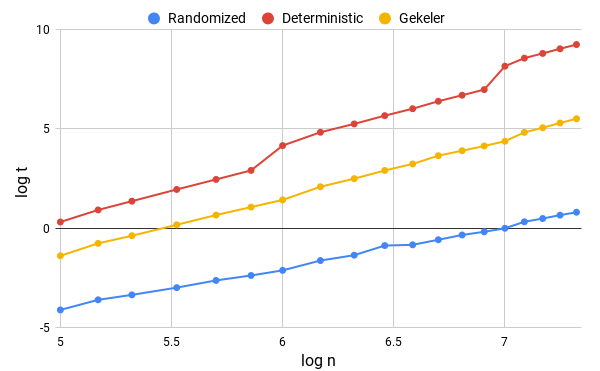
\includegraphics[width=3in]{chart-499-2.png}
  \caption{Log-log plot of $n$ versus runtime with $q = 499$, $m = 2$}
\end{figure}
    
\end{frame}

%--------------------------------------------------

\begin{frame}{Future Work}

Our main goal of achieving a sub-quadratic runtime in $n$ remains unfulfilled.

To this end, exploring whether additional elliptic techniques have efficient Drinfeld parallels may prove to be a fruitful topic of further investigation.




\end{frame}

%\begin{frame}
%\frametitle{References}
%\footnotesize{
%\begin{thebibliography}{99} % Beamer does not support BibTeX so references must be inserted manually as below
%\bibitem[Smith, 2012]{p1} M.B. Paterson, D.R. Stinson (2015)
%\newblock Combinatorial Characterizations of algebraic manipulation detection codes involving generalized difference families
%\end{thebibliography}
%}
%\end{frame}

%------------------------------------------------

%\begin{frame}
%\Huge{\centerline{Fin}}
%\end{frame}

%----------------------------------------------------------------------------------------

\end{document} 